\chapter{Расчет потокораспределения и напряжений в узлах сети в нормальном режиме наибольших нагрузок}
\label{cha:30-high_loads}

\section{Расчет нагрузок на шинах низшего и среднего напряжений подстанции}

Возьмем значения активной мощности на шинах низшего и среднего напряжений, $tg\varphi_\textup{н}$ и $cos\varphi_\textup{с}$ из табл. \ref*{tab:tabl2}.

Активная нагрузка на шинах низшего напряжения (НН): $P_\textup{н} = 22,9 \; \text{МВт}$

Реактивная нагрузка на шинах НН вычисляется по формуле:
\begin{eqndesc}
	\begin{equation*}
		Q_\textup{н} = P_\textup{н}\cdot tg\varphi_\textup{н} = 22,9\cdot 0,44 = 10,1\; \text{МВар},
	\end{equation*}

	где $P_\textup{н}$ "--- активная нагрузка на шинах НН; \\
	$tg_{\varphi_{\text{н}}}$ "--- коэффициент реактивной мощности.
\end{eqndesc}

Активная нагрузка на шинах среднего напряжения (СН): $P_\textup{с} = 33\; \text{МВт}$

Реактивная нагрузка на шинах СН:
\begin{eqndesc}
	\begin{equation*}
		Q_\textup{с} = \sqrt{S_c^2 - P_c^2} = \sqrt{\left(\frac{P_c}{cos\varphi_c}\right)^2 - P_c^2} = \sqrt{\left(\frac{33}{0,82}\right)^2 - 33^2} = 23,0\; \text{Мвар},
	\end{equation*}

	где $P_\textup{с}$ "--- активная мощность нагрузки на шинах СН; \\
	$cos_{\varphi_{\text{с}}}$ "--- коэффициент мощности нагрузки; \\
	$S_\textup{с}$ "--- полная мощность на шинах СН.
\end{eqndesc}


\section{Расчет режима наибольших нагрузок}

Найдем напряжение ИП-ПС:
\[U_\textup{ИП-ПС} = U_\textup{ном} \cdot U_\textup{ИП}, \% = 110\cdot 1,13 = 124,3\; \text{кВ}\]

\newpage
\textbf{1 этап}

В качестве начального приближения зададимся значениями напряжений на шинах СН и ВН, приведенными к стороне ВН, а так же напряжения в средней точке схемы замещения трансформатора (далее ТР), равными номинальному напряжению:
\[U_\textup{в}^{(0)} = U_\textup{н}^{{'}(0)} = U_\textup{с}^{{'}(0)} = U_0^{(0)} = U_\textup{ном} = 110\; \text{кВ}\]

\textbf{Луч среднего напряжения}

Мощность в конце луча СН:
\[S_c^{''} = P_c + jQ_c = 33,0 + j23,0 \; \text{МВА} \]

Потери мощности в сопротивлении по данным конца в общем виде рассчитываются по формуле:
\begin{eqndesc}[h]
	\begin{equation}
		\Delta S_{ij} = \left(\frac{S_{ij}^{''}}{U_{j}}\right)^2 \cdot Z_{ij}
		\label{eq:dS12}
	\end{equation}

	где $S_{ij}^{''}$ \--- мощность в конце участка \textit{i-j}, МВА, \\
	$U_j$ \--- напряжение в конце участка \textit{i-j}, кВ, \\
	$Z_{ij}$ \--- сопротивление участка \textit{i-j}, Ом.
\end{eqndesc}

Определим потери мощности в сопротивлении луча СН по формуле \eqref{eq:dS12}:
\[\Delta S_c = \frac{(S_c^{''})^2}{U_\textup{ном}^2}\cdot Z_c = \frac{33^2+23^2}{110^2}\cdot 0,413 = 0,055\; \text{МВт}\]

Определим мощность в начале луча СН:
\[S_c^{'} = S_c^{''} + \Delta S_c = 33,0 + j23,0 + 0,055 = 33,1 + j23,0\; \text{МВА}\]

\textbf{Луч низшего напряжения}

Мощность в конце луча НН:
\[S_\textup{н}^{''} = P_\textup{н} + jQ_\textup{н} = 22,9 + j10,1 \; \text{МВА}\]

Потери мощности в сопротивлении луча НН:
\[\Delta S_\textup{н} = \frac{(S_\textup{н}^{''})^2}{U_\textup{ном}^2}\cdot Z_\textup{н} = \frac{22,9^2+10,1^2}{110^2}\cdot (0,413 + j10,3) = 0,0214 + j0,533\; \text{МВА}\]

Определим мощность в начале луча НН:
\[S_\textup{н}^{'} = S_\textup{н}^{''} + \Delta S_\textup{н} = 22,9 + j10,1 + 0,0214 + j0,533 = 22,9 + j10,6 \; \text{МВА}\]

\textbf{Луч высшего напряжения}

Мощность в конце луча ВН:
\[S_\textup{в}^{''} = S_c^{'} + S_\textup{в}^{'} = 33,1 + j23,0 + 22,9 + j10,6 = 56,0 + j33,6 \; \text{МВА}\]

Потери мощности в сопротивлении луча ВН:
\[\Delta S_\textup{в} = \frac{(S_\textup{в}^{''})^2}{(U_\textup{ном})^2} \cdot Z_\textup{в} = \frac{56^2 + 33,6^2}{110^2} \cdot (0,413 + j17,9) = 0,146 + j6,31 \; \text{МВА} \]

Мощность в начале луча ВН:
\[S_\textup{в}^{'} = S_\textup{в}^{''} + \Delta S_\textup{в} = 56,0 + j33,6 + 0,146 + j6,31 = 56,1 + j39,9\; \text{МВА}\]

Приведенная нагрузка подстанции:
\[S_\textup{прив} = S_\textup{в}^{'} + \Delta S_\textup{х} = 56,1 + j39,9 + 0,086 + j0,48 = 56,2 + j40,4 \; \text{МВА}\]

Зарядная мощность в конце линии ИП-ПС:
\[\frac{Q_\textup{с.ИП-ПС}^{''}}{2} = \frac{U_\textup{ном}^2\cdot B_\textup{л}}{2} = \frac{110^2 \cdot 460,3\cdot 10^{-6}}{2} = 2,78\; \text{МВар} \]

Расчетная нагрузка подстанции:
\[S_p = S_\textup{прив} - j\frac{Q_\textup{с.ИП-ПС}^{''}}{2} = 56,2 + j40,4 - j2,78 = 56,2 + j37,6\; \text{МВА}\]

Мощность в конце линии ИП-ПС:
\[S_\textup{ИП-ПС}^{''} = S_p = 56,2 + j37,6\; \text{МВА}\]

Потери мощности в сопротивлении линии ИП:
\[\Delta S_\textup{ИП-ПС} = \frac{\left(S_\textup{ИП-ПС}^{''}\right)^2}{U_\textup{ном}^2}\cdot Z_\textup{л} = \frac{56,2^2 + 37,6^2}{110^2} \cdot (8,57 + j17,5) = 3,24 + j6,61 \; \text{МВА}\]

Мощность в начале линии ИП-ПС:
\[S_\textup{ИП-ПС}^{'} = S_\textup{ИП-ПС}^{''} + \Delta S_\textup{ИП-ПС} = 56,2 + j37,6 + 3,24 + j6,61 = 59,4 + j44,2 \; \text{МВА}\]

Зарядная мощность в начале линии ИП-ПС:
\[\frac{Q_\textup{с.ИП-ПС}^{'}}{2} = \frac{U_\textup{ИП-ПС}^2\cdot B_\textup{л}}{2} = \frac{124,3^2 \cdot 460,3\cdot 10^{-6}}{2} = 3,56\; \text{МВар}\]

Мощность, выдаваемая источником в сеть:
\[S_\textup{ИП-ПС} = S_\textup{ИП-ПС}^{'} - j\frac{Q_\textup{с.ИП-ПС}^{'}}{2} = 59,4 + j44,2 - j3,56 = 59,4 + 40,6\; \text{МВА}\]

\textbf{2 этап}

Продольная составляющая вектора падения напряжения по данным начала находится по формуле:

\begin{equation}
	\Delta U_{ij} = \frac{P_{ij}^{'}\cdot R_{ij} + Q_{ij}^{'}\cdot X_{ij}}{U_{i}}
\end{equation}

Поперечной составляющей можем пренебречь, так как линия класса напряжения 110 кВ.

Продольная составляющая вектора падения напряжения на сопротивлении линии ИП-ПС:
\[\Delta U_\textup{ИП-ПС} = \frac{P_\textup{ИП-ПС}^{'}\cdot R_\textup{л} + Q_\textup{ИП-ПС}^{'}\cdot X_\textup{л}}{U_\textup{ИП-ПС}} = \frac{59,4\cdot 8,57 + 44,2\cdot 17,5}{124,3} = 10,3\; \text{кВ}\]

Напряжение на шинах ВН:
\[U_\textup{в} = U_\textup{ИП-ПС} - \Delta U_\textup{ИП-ПС} = 124,3 - 10,3 = 114,0 \; \text{кВ}\]

Продольная составляющая вектора падения напряжения на сопротивлении луча высшего напряжения:
\[\Delta U_\textup{в} = \frac{P_\textup{в}^{'}\cdot R_\textup{т.в} + Q_\textup{в}^{'}\cdot X_\textup{т.в}}{U_\textup{в}} = \frac{56,1\cdot 0,413 + 39,9\cdot 17,9}{114,0} = 6,47\; \text{кВ}\]

Напряжение в средней точке cхемы замещения трансформаторов:
\[U_\textup{0} = U_\textup{в} - \Delta U_\textup{в} = 114,0 - 6,47 = 107,5 \; \text{кВ}\]

Продольная составляющая вектора падения напряжения на сопротивлении луча среднего напряжения:
\[\Delta U_\textup{с} = \frac{P_\textup{с}^{'}\cdot R_\textup{т.с} + Q_\textup{с}^{'}\cdot X_\textup{т.с}}{U_\textup{0}} = \frac{33,1\cdot 0,413 + 23,0\cdot 0}{107,5} = 0,127\; \text{кВ}\]

Напряжение на шинах СН, приведенное к стороне ВН:
\[U_\textup{с}^{'} = U_\textup{0} - \Delta U_\textup{н} = 107,5 - 0,127 = 107,4 \; \text{кВ}\]

Продольная составляющая вектора падения напряжения на сопротивлении луча низшего напряжения:
\[\Delta U_\textup{н} = \frac{P_\textup{н}^{'}\cdot R_\textup{т.н} + Q_\textup{н}^{'}\cdot X_\textup{т.н}}{U_\textup{0}} = \frac{22,9\cdot 0,413 + 10,6\cdot 10,3}{107,5} = 1,10\; \text{кВ}\]

Напряжение на шинах НН, приведенное к стороне ВН:
\[U_\textup{н}^{'} = U_\textup{0} - \Delta U_\textup{н} = 107,5 - 1,10 = 106,4 \; \text{кВ}\]

Полная расчетная схема замещения сети в нормальном режиме наибольшей нагрузки изображена на рис. \ref{fig:rezhim_NB}. 

\begin{sidewaysfigure}
	\centering
	\includegraphics[width=0.9\textwidth]{inc/svg/rezhim_NB}
	\caption{Полная схема замещения сети для режима наибольших нагрузок}
	\label{fig:rezhim_NB}
\end{sidewaysfigure}
%%% Local Variables:
%%% mode: latex
%%% TeX-master: "rpz"
%%% End: